\documentclass[twoside]{article}
\usepackage{graphicx, siunitx, float, polski, csquotes, pdfpages, chngcntr}
\usepackage[a4paper, top=2.5cm, bottom=2.5cm, inner=3.5cm, outer=2.5cm]{geometry}
\usepackage[hyphens]{url}
\usepackage[pdfusetitle]{hyperref}
\usepackage[backend=biber, sorting=none]{biblatex}
\usepackage[polish, english]{babel}

\addbibresource{sources.bib}
% \appto{\bibsetup}{\raggedright}
% \appto{\bibsetup}{\sloppy}
\hypersetup{hidelinks}
\counterwithin{figure}{section}
\renewcommand{\thefigure}{\thesection.\arabic{figure}}
\linespread{1.3}

\usepackage{subfiles}

\title{Budzik synchronizowany przez Wi-Fi}
\author{Wojciech Paderewski}

\begin{document}
\selectlanguage{polish}
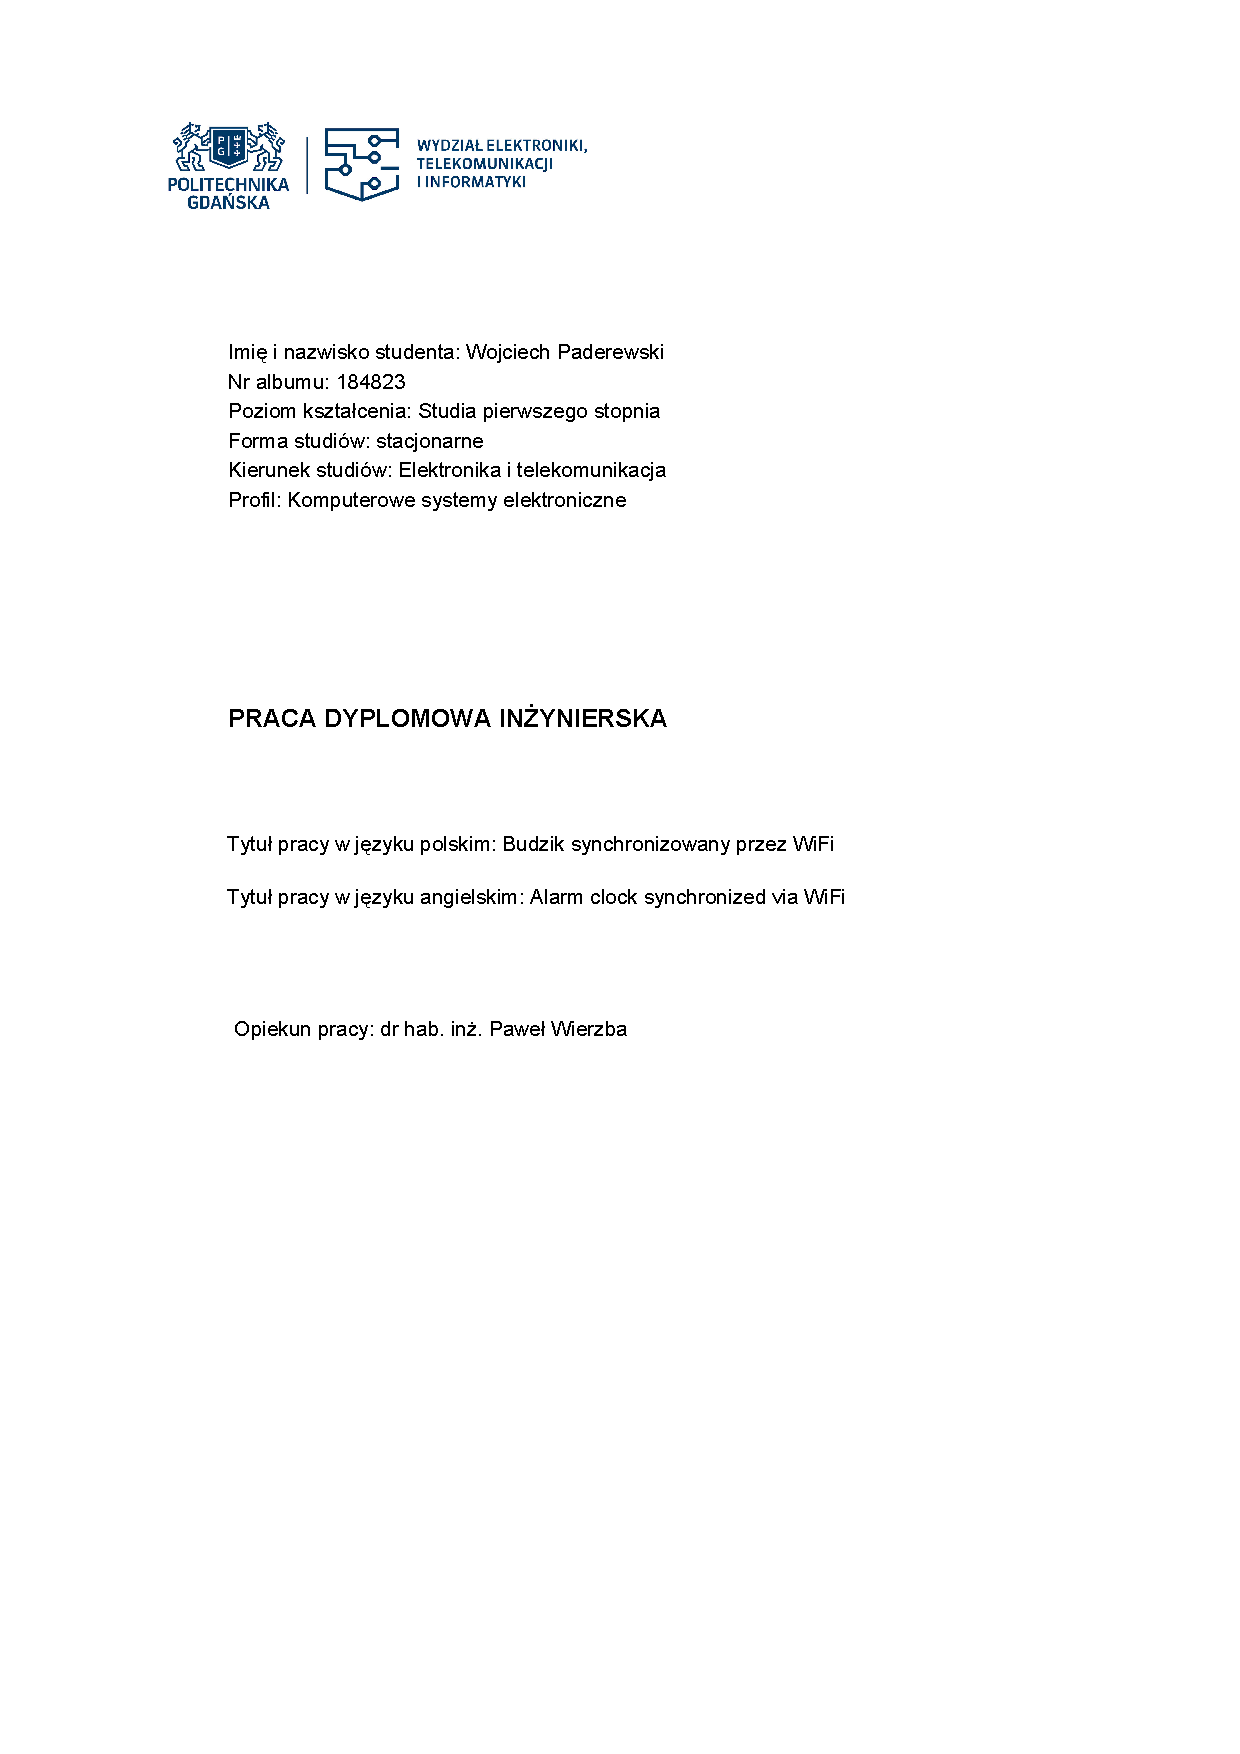
\includepdf[pages=1]{strona_tytulowa/strona_tytulowa.pdf}
\thispagestyle{empty}
\cleardoublepage

\subfile{abstrakt/abstrakt}
\cleardoublepage

\tableofcontents
\newpage
\subfile{skroty/skroty}
\cleardoublepage

\subfile{wstep/wstep}
\newpage
\subfile{koncepcja_ukladu/koncepcja_ukladu}
\newpage

\section{Budowa układu}
\subfile{budowa_ukladu/12V_to_5V_conv/12V_to_5V_conv}
\newpage
\subfile{budowa_ukladu/DC_Plug/DC_Plug}
\newpage
\subfile{budowa_ukladu/usb_c_to_program/usb_c_to_program}
\newpage

\printbibliography[]
\addcontentsline{toc}{section}{Bibliografia}
\newpage
\listoffigures
\addcontentsline{toc}{section}{Spis rysunków}
\newpage
\listoftables
\addcontentsline{toc}{section}{Spis tabel}
\end{document}
